\documentclass[12pt,a4paper,leqno]{report}

\usepackage[ansinew]{inputenc}
\usepackage[T1]{fontenc}
\usepackage[english]{babel}
\usepackage{amsthm}
\usepackage{amsfonts}         
\usepackage{amsmath}
\usepackage{amssymb}
\usepackage{enumitem}
\usepackage{fixltx2e}
\usepackage{tikz}
\usepackage{mathabx}
\usetikzlibrary{calc}



\newcommand{\argmax}{\operatornamewithlimits{argmax}}
\newcommand{\R}{\mathbb{R}}
\newcommand{\C}{\mathbb{C}}
\newcommand{\Q}{\mathbb{Q}}
\newcommand{\N}{\mathbb{N}}
\newcommand{\No}{\mathbb{N}_0}
\newcommand{\Z}{\mathbb{Z}}
\newcommand{\diam}{\operatorname{diam}}
\newcommand{\ob}{\operatorname{ob}}

\newcommand\opn{\mathrel{\ooalign{$\subset$\cr
			\hidewidth\hbox{$\circ\mkern.5mu$}\cr}}}
\newcommand\cls{\mathrel{\ooalign{$\subset$\cr
			\hidewidth\hbox{$c\mkern.5mu$}\cr}}}
\newcommand*{\QEDA}{\hfill\ensuremath{\blacksquare}}%

\theoremstyle{plain}
\newtheorem{lause}[equation]{Theorem}
\newtheorem{lem}[equation]{Lemma}
\newtheorem{prop}[equation]{Proposition}
\newtheorem{kor}[equation]{Corollary}
\newtheorem{vaite}{V�ite}

\setcounter{secnumdepth}{3}
\newcounter{diagram}
\numberwithin{diagram}{subsection}
\newenvironment{diagram}
{\stepcounter{diagram}\par\smallskip\noindent\begin{minipage}{\linewidth}\centering}
	{\par Diagram~\thediagram\end{minipage}\par\smallskip}
\theoremstyle{definition}
\newtheorem{maar}[equation]{Definition}
\newtheorem{konj}[equation]{Conjecture}
\newtheorem{esim}[equation]{Example}

\theoremstyle{remark}
\newtheorem{huom}[equation]{Huomautus}

\pagestyle{plain}
\setcounter{page}{1}
\addtolength{\hoffset}{-1.15cm}
\addtolength{\textwidth}{2.3cm}
\addtolength{\voffset}{0.45cm}
\addtolength{\textheight}{-0.9cm}


\title{Cech (co)homology}
\author{Yury Elkin}
\date{}



\begin{document}

\maketitle

\tableofcontents

\chapter{Inroduction}\label{johd}



\chapter{Background}

In this chapter we will recall a few details about algebra, category theory and abstract simplicial complexes. We assume that the reader is familiar with basic concepts of homology and cohomology theory and constructions related to them.

\section{Direct sum and direct product}
In this section we will recall a few details about direct sums and direct products.
\begin{maar}
Let $\{A_i\}_{i \in J}$ be a family of groups. The direct product of these groups is the Cartesian product $\prod_{i \in J} A_i$ where addition is defined component-wise $(a+b)_i = a_i+_ib_i$
\end{maar}
\begin{maar}
Let $\{A_i\}_{i \in J}$ be a family of groups. The direct sum of these groups is the subgroup of direct product given by  $\bigoplus_{i \in J}A_i = \{x \in \prod_{i \in J} A_i \mid x_i \neq 0 \text{ for only finetely many } i \}. $
\end{maar}
For direct sums and direct products we have following universal properties:
\begin{lem}\label{Universalpropertyproduct}
Let $A = \prod_{i \in J} A_i$ be the direct sum and $D$ an arbitrary group. Then for every set of homomorphisms $\{f_i:D \rightarrow A_i\}_{i \in J}$ there exists a unique homomorphism $f:D \rightarrow A$ for which condition $pr_i \circ f = f_i $ holds for every $i \in J$.
\end{lem}
\begin{proof}
Proved in [\ref{algebra2}] theorem 3.7.
\end{proof}
\begin{lem}\label{Universalpropertysum}
	Let $A = \bigoplus_{i \in J}A_i$ be direct sum and $D$ arbitary group. Then for every set homomorphisms $\{f_i:A_i \rightarrow D\}_{i \in J}$ there exists unique homomorphism $f:A \rightarrow D$ for which and for every $i \in J$ condition $ f \circ j_i = f_i $ holds.
\end{lem}
\begin{proof}
Proved in [\ref{algebra2}] theorem 3.6.
\end{proof}
\section{Category theory}

In this thesis we will present theory in a categorical way, which will make the construction more general. First lets recall the definition of a category. 

\begin{maar}
A category C consist of the following ingredients: A class of objects $\ob(C)$, a class of morphisms $\hom(C)$ for which and for every objects $A$, $B$ in $\ob(C)$ there exists a subclass $Hom(A,B)$ and a rule of composition $Comp:Hom(A,B) \times Hom(B,D) \rightarrow Hom(A,D)$ for which following conditions hold:
\begin{enumerate}[label=(\arabic*),ref=(\arabic*)]
	
	
	\item Composition is associative. Let $f:A \rightarrow B$, $g: B \rightarrow D$ and $h: D \rightarrow E$ be morphisms between objects then $(f \circ g) \circ h = f \circ (g \circ h)$
	
	\item For every object $A \in \ob(C)$ there exists identity morphism $1_A \in \hom(A,A)$ for which the following condition holds: Let $f:A \rightarrow B$ and $g: B \rightarrow A$ be arbitrary morphisms then $f \circ 1_A = f$ and $1_A \circ g = g$.
	
\end{enumerate}
\end{maar}
It is easy to see that topological spaces with continuous functions and abelian groups with homomorphisms form a category. We denote those categories by TOP and AB. Next we will define the concept of a functor between categories.
\begin{maar}
Let $C$ and $C'$ be categories and $F$ map between them. We say that $F$ is functor between categories if the following conditions hold:

\begin{enumerate}[label=(\arabic*),ref=(\arabic*)]
	
	
	\item For every object $A \in \ob(C)$ there exists a unique object $F(A) \in C'$.
	
	\item Let $A$ and $B$ be objects in $\ob(C)$ and $f:A \rightarrow B$ a morphism between them. Then there exists a unique morphism $F(f):F(A) \rightarrow F(B)$.
	
	\item if $f$ and $g$ are morphisms in $\hom(C)$, then the following condition holds: $F(f) \circ F(g) = F(f \circ g)$.
	
	\item The identity element is mapped to the identity element. Let $A$ be an object in $\ob(C)$ and $1_A$ the identity morphism corresponding to it. Then $F(1_A)$ is identity morphism of $F(A)$.
		

\end{enumerate}

\end{maar}
Homology and cohomology groups form a functor from TOP to AB. For details see Rotman [\ref{rotman}]. Now we will introduce a new concept called natural transformation.

\begin{maar}
Let $C$ and $D$ be categories and $F:C \rightarrow D$ and $G:C \rightarrow D$ functors between them. Then the following family of functors is a natural transformation: $$\{\phi_X: F(X) \rightarrow G(X)\}_{X \in C}$$ 
if the following conditions hold:
\begin{enumerate}[label=(\arabic*),ref=(\arabic*)]
	
	
	\item For every object $X \in C$ there exists a unique morphism $\phi_X: F(X) \rightarrow G(X) $
	
	\item For every morphism $f:X \rightarrow Y$ the following diagram commutes:
	
	$$ 	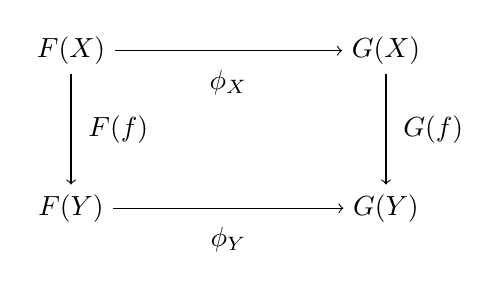
\begin{tikzpicture}
	
	
	
	\node (w) at (0,0) {\(F(X)\)};
	
	\node (x) at (0,-2) {\(F(Y)\)};
	
	\node (y) at (4,-2) {\(G(Y)\)};
	
	\node (z) at (4,0) {\(G(X)\)};
	
	\node (f) at (2,-2.4){\(\phi_Y\)};
	
	\node (g) at (2,-0.4){\(\phi_X\)};
	
	\node (s) at (0.6,-1) {\(F(f)\)};
	
	\node (s2) at (4.6,-1) {\(G(f)\)};	
	
	\draw[->] (z) -- (y);
	\draw[->] (w) -- (x);
	\draw[->] (x) -- (y);
	\draw[->] (w) -- (z);
	
	
	\end{tikzpicture}
	$$
	
	or in other words $\phi_Y \circ F(f) = G(f) \circ \phi_X $ holds.
	
\end{enumerate}
\end{maar}


Next we will define the concepts of limit and colimit for arbitrary categories, which will be later applied to directed and inverse systems.

\begin{maar}
Let $C$ be an indexed category in such a way that there exists a category $J$ with a functor $F:J \rightarrow C$. Let $N$ be fixed object of $\ob(C)$. We define the cone from $N$ to $F$ to be an indexed family of morphisms $$\{\omega_X: N \rightarrow F(X)\}_{X \in J}$$ which satisfies following property: If $f:X \rightarrow Y$ is a morphism in $C$ then the following diagram commutes


$$
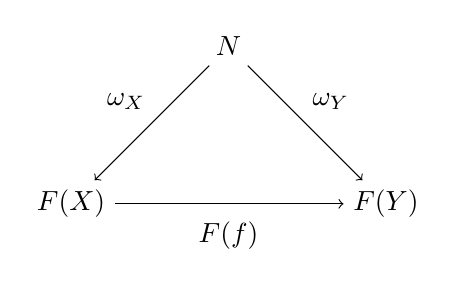
\begin{tikzpicture}

\node (w) at (2,0) {\(N\)};

\node (x2) at (0.7,-0.7) {\(\omega_X\)};

\node (x) at (0,-2) {\(F(X)\)};

\node (y2) at (3.3,-0.7) {\(\omega_Y\)};

\node (y) at (4,-2) {\(F(Y)\)};

\node (f) at (2,-2.4){\(F(f)\)};


\draw[->] (w) -- (y);
\draw[->] (w) -- (x);
\draw[->] (x) -- (y);


\end{tikzpicture}
$$
We denote this structure by $(N, \omega)$.
\end{maar}

\begin{maar}
Let $C$ be an indexed category which is indexed by a category $J$ and a functor $F$. Let $f:X \rightarrow Y$ be arbitrary morphism in category $J$ and let $D$ be an object of the category $C$ which forms a cone together with a family of morphisms $\{\phi_X\}_{X \in \ob(C)}$ and morphism $f$. We say that $(D, \phi)$ is a limit of $C$ if the following property holds: If $N$ together with family $\{\omega_X\}_{X \in \ob(C)} $ and morphism $f$ is any other cone of category $C$, then there exists a unique morphism $u:N \rightarrow D$ in such way that the following diagram commutes:
\end{maar} 
$$
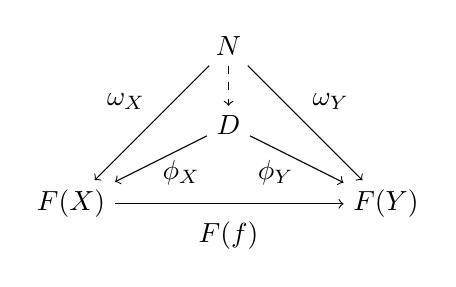
\begin{tikzpicture}

\node (w) at (2,0) {\(N\)};

\node (x2) at (0.7,-0.7) {\(\omega_X\)};

\node (x) at (0,-2) {\(F(X)\)};

\node (y2) at (3.3,-0.7) {\(\omega_Y\)};

\node (y) at (4,-2) {\(F(Y)\)};

\node (f) at (2,-2.4){\(F(f)\)};

\node (d) at (2,-1){\(D\)};

\node (phid) at (1.4,-1.6){\(\phi_X\)};
\node (phid2) at (2.6,-1.6){\(\phi_Y\)};


\draw[->] (w) -- (y);
\draw[->] (w) -- (x);
\draw[->] (x) -- (y);
\draw[dashed][->] (w) -- (d);
\draw[->] (d) -- (x);
\draw[->] (d) -- (y);


\end{tikzpicture}
$$
Next we will prove that if we have two limits $N$ and $D$ of a category $C$ then there exists an isomorphism between those two objects. In other words $N$ and $D$ can be identified and the limit of category $C$ can be denoted simply as $\displaystyle {\lim_\rightarrow C}$ .

\begin{lause}
Let $N$ and $D$ be limits of a category $C$. Then there exists an isomorphism between them.
\end{lause}
\begin{proof}
Because $N$ and $D$ are both limits there exists morphisms $u: N \rightarrow D$ and $v: D \rightarrow N $. Because of the symmetry it is enough $u \circ v = id_N$. This follows from equations $\omega_X \circ u \circ v  = \phi_X \circ u = \omega_X$ and $u \circ v \circ \omega_Y = u \circ \phi_Y = \omega_Y$. Because the diagram commutes for $id_N$ then by the uniqueness condition we see that $u \circ v = id_N$. 
\end{proof}
\subsection{Dual category}
To simplify definitions we will define the concept of dual category. In this section we will interpret category as a model of first order logic
\begin{maar}
Let $\omega$ be a statement in this model. We get a dual statement $\omega^{op}$ by following procedure:

\begin{enumerate}[label=(\arabic*),ref=(\arabic*)]
	
	\item Interchange every occurrence of source with target
	\item Reorder every composition. That is replace $a \circ b$ with $b \circ a$.
	
\end{enumerate}
%% Tarkistus suoritettu t�h�n asti
\end{maar}
Next we will give an important example of a dual statement. 
\begin{maar}
The colimit of a category $C$ is the dual statement of limit of $C$. We define the cocone to be dual of cone. Let $J$ be index category of $C$ then we say that a cocone induced by $D$ is the colimit of category $C$ if for every other cocone induced by $N$ there exists a unique morphism $u:D \rightarrow N$ in such a way that the diagram below commutes:
$$
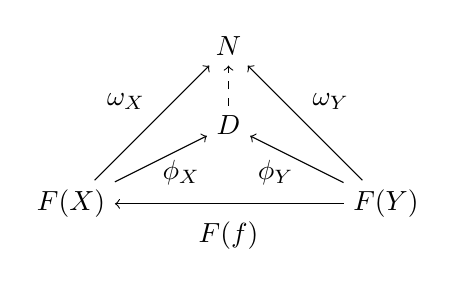
\begin{tikzpicture}

\node (w) at (2,0) {\(N\)};

\node (x2) at (0.7,-0.7) {\(\omega_X\)};

\node (x) at (0,-2) {\(F(X)\)};

\node (y2) at (3.3,-0.7) {\(\omega_Y\)};

\node (y) at (4,-2) {\(F(Y)\)};

\node (f) at (2,-2.4){\(F(f)\)};

\node (d) at (2,-1){\(D\)};

\node (phid) at (1.4,-1.6){\(\phi_X\)};
\node (phid2) at (2.6,-1.6){\(\phi_Y\)};


\draw[->] (y) -- (w);
\draw[->] (x) -- (w);
\draw[->] (y) -- (x);
\draw[dashed][->] (d) -- (w);
\draw[->] (x) -- (d);
\draw[->] (y) -- (d);


\end{tikzpicture}
$$
\end{maar}
Like limits colimits are unique. 

\begin{lause}
Let $N$ and $D$ be colimits of category $C$. Then there exists isomorphism between them.
\end{lause}
\begin{proof}
Because $N$ and $D$ are both colimits there exist morphisms $u: N \rightarrow D$ and $v: D \rightarrow N $. Because of the symmetry it is enough $u \circ v = id_N$. This follows from equations: $u \circ v \circ \omega_X = u \circ \phi_X = \omega_X$ and $u \circ v \circ \omega_Y = u \circ \phi_Y = \omega_Y$. Because the diagram commutes for $id_N$ by uniqueness condition we see that $u \circ v = id_N$. 
\end{proof}
\subsection{Direct and inverse systems}
In this section we will give a categorical definition of direct and inverse systems. It appears that those concepts are dual of each other. We will begin by defining quasi-ordering relation:

\begin{maar}
Let $a \leq b$ be a relation in a set $\lambda$. We say that this relation is a quasi-ordering if the following conditions hold:
\begin{enumerate}[label=(\arabic*),ref=(\arabic*)]
	
	
	\item $a \leq a$ for all $a \in \lambda$
	\item if $a \leq b$ and $b \leq c$ then $a \leq c$ for all $a,b,c \in \lambda$
	
\end{enumerate}

\end{maar}
\begin{maar}
Let $\lambda$ be quasi-ordered set and $\mathcal{L}$ a category then a direct $\lambda$-system consist of functor $D$ which assigns unique object $D(\lambda) \in \mathcal{L}$ and a family of morphism in such way that for every pair $a \leq b$ there exists unique morphism $D^b_a: D(a) \rightarrow D(b)$. The family of morphisms satisfies following conditions:

\begin{enumerate}[label=(\arabic*),ref=(\arabic*)]
	
	\item For every triple $a \leq b \leq c$ in $\lambda$ functions commute in a following way: $D^c_b \circ D^b_a = D^c_a$
	\item For every $a \in \lambda$: $D^a_a = id_a$
	
\end{enumerate}

\end{maar}

The structure in above definition can be also viewed as category $C$ in such way that $\ob(C) = D(\lambda)$ and for every $D(a),D(b) \in \ob(C)$ there exists exactly one morphism in $\hom(D(a),D(b)$. In other words $\lambda$ is indexation of subcategory of $\mathcal{L}$. We can define dual concept of above definition in a following way:

\begin{maar}
Let $\lambda$ be quasi-ordered set and $\mathcal{L}$ category. Then inverse system is dual of a direct system. Let $I$ be functor from $\lambda$ to $\mathcal{L}$ in such way that for every pair $a \leq b$ there exists unique morphism $I^b_a: I(b) \rightarrow I(a)$ and following properties hold: $I^c_b \circ I^b_a = I^c_a$ and $I^a_a = id_a$.
\end{maar}

\begin{esim}
Let SET be category of sets with order relation in such way that $U \leq V \Leftrightarrow U \subset V$ now for every $U,V$ we define $D_U^V U \rightarrow V $ to be just inclusion from $U$ to $V$. Clearly this forms direct system. 
\end{esim}

Next we define a bit more complex category 

\begin{maar}
Direct systems together with natural transformations between them form Category. We will denote elements of this category shortly $(\lambda, \mathcal{L})$
\end{maar}
Taking dual and using functor $I$ instead of $D$ we see that natural transformation with inverse system form category. We will denote this category by $(\lambda, \mathcal{L}^{op})$. Now we can define limit of the category $(\lambda, \mathcal{L})$. We see that for every quasi-order $\lambda$ and object $k$ in $\mathcal{L}^{op}$ we can define inverse system by mapping every element $\lambda$ to the object $k$ and every functor between objects in $\lambda$ to identity functor. This forms inverse system which we will denote by $K$. Now natural transformations $\phi_a : D(a) \rightarrow K$ between $K$ and arbitrary element in $(\lambda, \mathcal{L})$ induces following: co(cone) 
$$
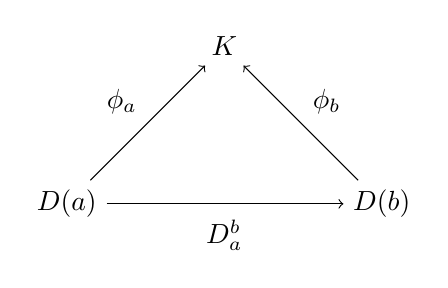
\begin{tikzpicture}

\node (w) at (2,0) {\(K\)};

\node (x2) at (0.7,-0.7) {\(\phi_a\)};

\node (x) at (0,-2) {\(D(a)\)};

\node (y2) at (3.3,-0.7) {\(\phi_b\)};

\node (y) at (4,-2) {\(D(b)\)};

\node (f) at (2,-2.4){\(D^b_a\)};


\draw[->] (y) -- (w);
\draw[->] (x) -- (w);
\draw[->] (x) -- (y);


\end{tikzpicture}
$$
So we can define (co)limit of this structure in unique way if it exists. We will now give important example of this construction and show that in case category is $AB$ there exists such limit. To prove this result we first recall following lemma:


\begin{lause}
Let $D:\lambda \rightarrow AB$ be a direct system of groups. Let $G$ be the subgroup of $\bigoplus_{a \in \lambda} D(a) $ with is generated by $\{i_ax_{a}-i_bD^b_ax_a\}$. Then limit of this system is $L = \bigoplus_{a \in \lambda} D(a) / G $
\end{lause}
\begin{proof}
Let $\{v_a:D(a) \rightarrow L\}$ induce cone $L$ and $K$ be any other cocone induced by functors $\{\phi_a:D(a) \rightarrow K\}$. We have to prove that there exists unique homomorphism $u:L \rightarrow K$ for which condition $u \circ v_a = \phi_a $ holds for all $a \in \ob(\mathcal{L})$. Lets first assume that such homomorphism exists and prove that it is unique. Because images of functors $v_a$ generate space $L$ it follow that $u$ must be unique  \newline
We will now construct morphism $u$. Using lemma \ref{Universalpropertysum} we can find unique homomorphism $u':\bigoplus_{a \in \lambda} D(a) \rightarrow K$ for which $u' \circ i_a = \phi_a$ holds. Now we see that for every generator of subgroup G $u'(i_ax_{a}-i_bD^b_ax_a) = \phi_a(x_a) - \phi_bD_a^bx_a = \phi_a(x_a)-\phi_a(x_a) = 0$. Now we can define $u$ in such way that every element $x + D$ maps to element $\phi'(x)$. We will denote the projection map from $\bigoplus_{a \in \lambda} D(a)$ to $L$ by $p$. Now we see that $u \circ v_a = u \circ p \circ i_a = u' \circ i_a = \phi_a $.
\end{proof}
\begin{lause}
Let $I: \lambda \rightarrow AB$ be a inverse system of groups. Then limit of this system is group $L = \{x \in \prod_{i \in J} I_i \mid x_a = I^b_ax_b $ for all $a \leq b\}$
\end{lause}
\begin{proof}
Let $\{v_a: L \rightarrow I(a)\}_{a \in \lambda}$ induce cone $L$ and $K$ be any other cone induced by functors $\{\phi_a: K \rightarrow I(a)\}_{a \in \lambda}$. We construct function $u: K \rightarrow L$ for which $v_a \circ u = \phi_a$. By lemma \ref{Universalpropertyproduct} we know that there exists unique homomorphism $u':K \rightarrow \prod_{i \in J}I_i$ for which $pr_a \circ u' = \phi_a$. It is easy to see that $u'$ maps actually every element to $L$. Assume that $\beta$ and $\alpha$ are elements which satisfy $a \leq b$ condition. Then $I^{a}_b \circ pr_b \circ u'= I^{a}_b \circ \phi_b = \phi_a = pr_a \circ u'$. We can define $u$ to be $u'$.
\end{proof}

\subsection{Morphisms between systems}\label{limitmorphism}
\subsubsection{Morphisms between inverse systems}

To be able to define morphisms between Cech homology groups we need concept of limit homomorphism. In this section we will define limit morphism between systems and investigate properties of it. Concepts used in this chapter can be presented in more general case. However, for our use case its enough to restrict ourselves to the category of Abelian groups.

\begin{maar}
Functor $\phi:X \rightarrow Y$ is order preserving if for every elements $a$ and $b$ in set $X$ for which $a \leq b$, the condition $\phi(a) \leq \phi(b)$ is satisfied.
\end{maar}

We recall that we interpret inverse and direct systems as functors from the category $\lambda$ to some specific category. Let $I$ be inverse system and $\phi: \lambda' \rightarrow \lambda$ order preserving functor. Then inverse system $(I \phi, \lambda' )$ consist of objects $\{I'(\phi(a)) \mid a \in \lambda'\}$ and morphisms $\{I^{\phi(b)}_{\phi(a)}\mid a \leq b \}$.

\begin{maar}
Let $(I,\lambda)$ be inverse system and $\phi: \lambda' \rightarrow \lambda$ some functor. Let $(I \phi, \lambda' )$ be inverse system described above. Then we say $\phi$ is limit preserving functor, if it satisfies $\phi(I^{-1}(\lim I)) = I^{-1}(\lim(I \phi) )$ \footnote{Because we defined $\phi$ to be functor between $\lambda$ and $\lambda'$ we have to use functo $I^{-1}$, which is well-defined because of bijectivity of functor $I$. }
\end{maar}

\begin{maar}
Let $(I,\lambda)$ and $(I',\lambda')$ be inverse systems and $\phi:\lambda' \rightarrow \lambda$ an order and limit preserving functor. Let $ \{f_a:I(\phi(a)) \rightarrow I'(a) \mid a \in \lambda\}$ be natural transformation between $I\phi$ and $I'$. Then we say that $\{f_a\}_{a \in \lambda}$ is an inverse system of morphisms corresponding to functor $\phi$ of the system $I$ into system $I'$.
\end{maar}

In next theorem we prove that it is possible to define limit of the morphism between systems in an unique way. We recall that exists of limit implies that for every objects of category $I$ there exists unique functor $u_{I,a}:\lim I \rightarrow I(a)$.

\begin{lem}
Let  $(I,\lambda)$ and $(I',\lambda')$ be inverse systems for which limit exists. Let $\{f_a\}$ be inverse system of morphisms corresponding to that pair. Then there exists unique morphism $\lim f:\lim I \rightarrow \lim I'$ for which and for every $a \in \lambda'$ condition $\lim f \circ u_{I, \phi(a)} = u_{I',a} \circ f_a$ holds.
\end{lem}
\begin{proof}
Consider following diagram
\begin{diagram}\label{morphismbetweenlimits}
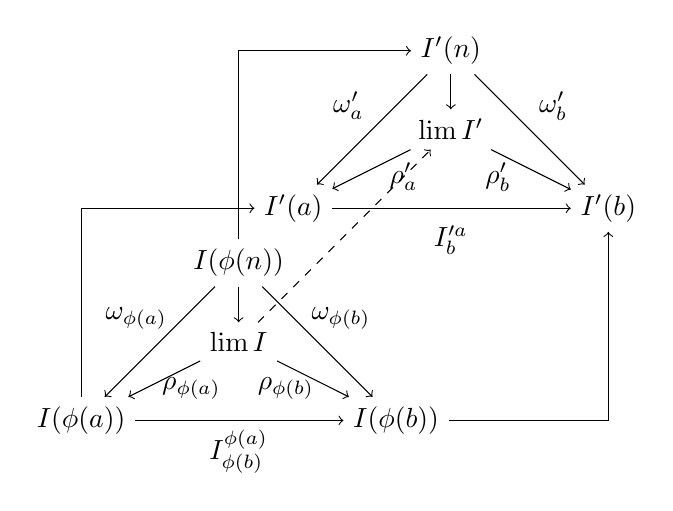
\begin{tikzpicture}



\node (w) at (2,0,0) {\(I(\phi(n))\)};

\node (x2) at (0.7,-0.7,0) {\(\omega_{\phi(a)}\)};

\node (x) at (0,-2,0) {\(I(\phi(a))\)};

\node (y2) at (3.3,-0.7,0) {\(\omega_{\phi(b)}\)};

\node (y) at (4,-2,0) {\(I(\phi(b))\)};

\node (f) at (2,-2.4,0){\(I^{\phi(a)}_{\phi(b)}\)};

\node (d) at (2,-1,0){\(\lim I\)};

\node (phid) at (1.4,-1.6,0){\(\rho_{\phi(a)}\)};
\node (phid2) at (2.6,-1.6,0){\(\rho_{\phi(b)}\)};

\node (w2) at (2,0,-7) {\(I'(n)\)};

\node (x22) at (0.7,-0.7,-7) {\(\omega'_a\)};

\node (x2) at (0,-2,-7) {\(I'(a)\)};

\node (y22) at (3.3,-0.7,-7) {\(\omega'_b\)};

\node (y2) at (4,-2,-7) {\(I'(b)\)};

\node (f2) at (2,-2.4,-7){\(I'^{a}_{b}\)};

\node (d2) at (2,-1,-7){\(\lim I'\)};

\node (phid2) at (1.4,-1.6,-7){\(\rho'_a\)};
\node (phid22) at (2.6,-1.6,-7){\(\rho'_b\)};

\draw[->] (w) -- (y);
\draw[->] (w) -- (x);
\draw[->] (x) -- (y);
\draw[->] (w) -- (d);
\draw[->] (d) -- (x);
\draw[->] (d) -- (y);

\draw[->] (w2) -- (y2);
\draw[->] (w2) -- (x2);
\draw[->] (x2) -- (y2);
\draw[->] (w2) -- (d2);
\draw[->] (d2) -- (x2);
\draw[->] (d2) -- (y2);

\draw[->] (w) |- (w2);
\draw[->] (x) |- (x2);
\draw[->] (y) -| (y2);


\draw[dashed][->](d) -- (d2);


\end{tikzpicture}
\end{diagram}

To prove that the limit morphism exists we form following triangle out of the diagram described above:

$$
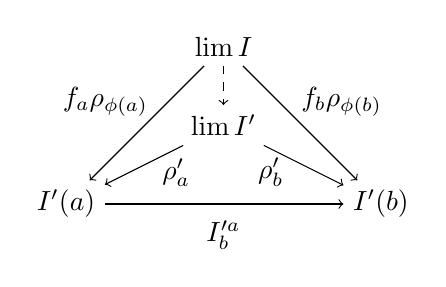
\begin{tikzpicture}

\node (w) at (2,0) {\(\lim I\)};

\node (x2) at (0.5,-0.7) {\(f_a \rho_{\phi(a)}\)};

\node (x) at (0,-2) {\(I'(a)\)};

\node (y2) at (3.5,-0.7) {\(f_b \rho_{\phi(b)}\)};

\node (y) at (4,-2) {\(I'(b)\)};

\node (f) at (2,-2.4){\(I'^{a}_{b}\)};

\node (d) at (2,-1){\(\lim I'\)};

\node (phid) at (1.4,-1.6){\(\rho'_a\)};
\node (phid2) at (2.6,-1.6){\(\rho'_b\)};


\draw[->] (w) -- (y);
\draw[->] (w) -- (x);
\draw[->] (x) -- (y);
\draw[dashed][->] (w) -- (d);
\draw[->] (d) -- (x);
\draw[->] (d) -- (y);


\end{tikzpicture}
$$
Then by definition of limit there exists unique morphism $\lim f:\lim I \rightarrow \lim I'$ for which the diagram commutes. We will prove now that the universal property $\lim f \circ u_{I, \phi(a)} = u_{I',a} \circ f_a$ holds for limit morphism. By diagram \ref{morphismbetweenlimits} and fact that the family of function $\{f_a\}$ is natural transformation or in other words condition $\omega'_a \circ f_n = f_a \circ \omega_{\phi(a)}$ holds following diagram commutes:
$$
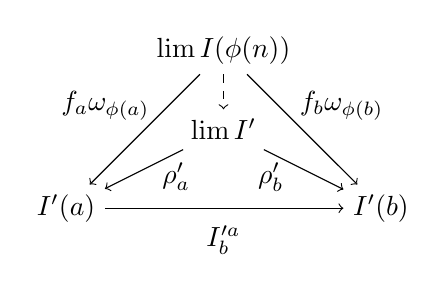
\begin{tikzpicture}

\node (w) at (2,0) {\(\lim I(\phi(n))\)};

\node (x2) at (0.5,-0.7) {\(f_a \omega_{\phi(a)}\)};

\node (x) at (0,-2) {\(I'(a)\)};

\node (y2) at (3.5,-0.7) {\(f_b \omega_{\phi(b)}\)};

\node (y) at (4,-2) {\(I'(b)\)};

\node (f) at (2,-2.4){\(I'^{a}_{b}\)};

\node (d) at (2,-1){\(\lim I'\)};

\node (phid) at (1.4,-1.6){\(\rho'_a\)};
\node (phid2) at (2.6,-1.6){\(\rho'_b\)};


\draw[->] (w) -- (y);
\draw[->] (w) -- (x);
\draw[->] (x) -- (y);
\draw[dashed][->] (w) -- (d);
\draw[->] (d) -- (x);
\draw[->] (d) -- (y);


\end{tikzpicture}
$$
Both maps $\lim f \circ u_{I, \phi(a)}$ and $u_{I',a} \circ f_a$ complete the diagram. Thus by uniqueness of the map corresponding to limit, we can conclude that the functions are same.

\end{proof}
For composition of two limits we have following result:

\begin{lem}
Let $(I, \lambda)$, $(I',\lambda')$ and $(I'',\lambda'')$ be inverse systems with limits and let $\phi:\lambda' \rightarrow \lambda$ and $\phi':\lambda'' \rightarrow \lambda'$ functors between systems. Let $ \{f_a:I(\phi(a)) \rightarrow I'(a) \mid a \in \phi'(\lambda'')\}$ and $ \{g_a:I'(\phi(a)) \rightarrow I''(a) \mid a \in \lambda''\}$ be family of morphisms corresponding to $\phi$ and $\phi'$. Let $\lim(f \circ g):I \rightarrow I''$ be limit of the family $\{g_af_{\phi(a)}:I(\phi \phi'(a)) \rightarrow I''(a) \mid a \in \lambda''\}$.  Then $\lim(f \circ g) = \lim f \circ \lim g $ holds.
\end{lem}
\begin{proof}
To prove this we will use previous lemma and following commutable diagram:
	$$
	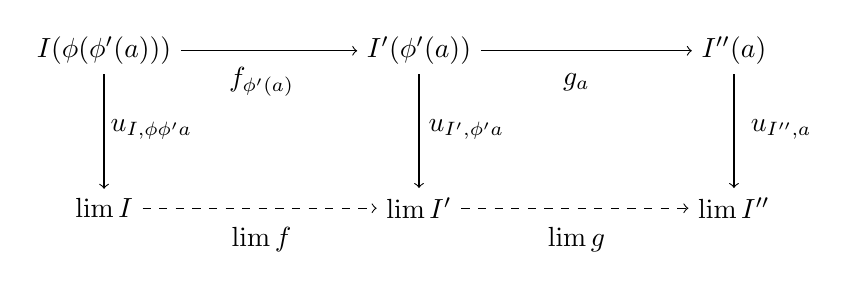
\begin{tikzpicture}
	
	
	
	\node (w) at (0,0) {\(I(\phi(\phi'(a)))\)};
	
	\node (x) at (0,-2) {\(\lim I\)};
	
	\node (y) at (4,-2) {\(\lim I'\)};
	
	\node (z) at (4,0) {\(I'(\phi'(a))\)};
	
	\node (p) at (8,0) {\(I''(a)\)};
	
	\node (p2) at (8,-2) {\(\lim I''\)};
	
	\node (f) at (2,-2.4){\(\lim f\)};\
	
	\node (f2) at (6,-2.4){\(\lim g\)};
	
	\node (g) at (2,-0.4){\(f_{\phi'(a)}\)};
	
	\node (g2) at (6,-0.4){\(g_{a}\)};
	
	\node (s) at (0.6,-1) {\(u_{I,\phi \phi'a}\)};
	
	\node (s2) at (4.6,-1) {\(u_{I', \phi'a}\)};	
	
	\node (s3) at (8.6,-1) {\(u_{I'', a}\)};	
	
	\draw[->] (z) -- (y);
	\draw[->] (w) -- (x);
	\draw[dashed][->] (x) -- (y);
	\draw[->] (w) -- (z);
	\draw[dashed][->] (y) -- (p2);
	\draw[->] (p) -- (p2);
	\draw[->] (z) -- (p);
	
	
	\end{tikzpicture}
	$$
	By definition of limit morphism condition $\lim (f \circ g) \circ u_{I, \phi(\phi'(a))} = u_{I'',a} \circ (g_a \circ f_{\phi(a)})$ holds for limit of the composition. By uniqueness of limit homomorphism it is enough to show that the composition of two limit functors satisfies the condition. This follows from following equations:
	$$\lim g \circ \lim f \circ u_{I, \phi(\phi'(a))} = \lim g  \circ u_{I, \phi'(a)} \circ f_{\phi'(a)} = u_{I'',a} \circ g_a \circ f_{\phi(a)} $$
	

\end{proof}

Now we would like to define limit for the system of homomorphisms between inverse systems of groups.

\begin{lem}\label{limitmorphismgroup}
Let $(I, \lambda)$ and $(I',\lambda')$ be inverse systems of groups. Then $$f:\lim_{\rightarrow} I \rightarrow \lim_{\rightarrow}I' : f(x) = \prod_{a \in \lambda}f_a(proj_{\phi(a)}(x))$$
is well defined function between limit groups.
\end{lem}
\begin{proof}
We have to show that the image is in the subgroup $$L = \{x \in \prod_{i \in \lambda'} I'(i) \mid x_a = I^b_ax_b \text{ for all } a \leq b \}.$$ Let $b$ be some index, then: $I'^{b}_{a}x'_b = I'^{b}_{a}f_b(x_{\phi(b)}) = f_bI'^{\phi(b)}_{\phi(a)}(x_{\phi(b)}) = f_ax_{\phi(a)} = x'_a$ . In this equation we used property which says that the morphisms define natural transformation.
\end{proof}

\subsection{Finality properties of subsystems}
Final and cofinal functors can be defined in a categorical way. However, for our purpose it is enough to investigate finality in special case of the category being system.


%% continue here:
\begin{maar}
Let $\lambda$ be a category with quasi-order relation on its objects and let $\omega$ be its subcategory. Then we say that $\omega$ is cofinal subcategory of $\lambda$, if for every element $a \in \ob(\lambda)$ there exist 
\end{maar}

\begin{maar}
Let $\lambda$ be category, the objects of which are induced by quasi-ordered set $\lambda$ and let $A$ be its subcategory. The subcategory $A$ is cofinal subset of $C$ if for every element $\beta \in X$ we can find element $\alpha \in A$ for which condition $\beta \leq \alpha$ holds.
\end{maar}
Now for inverse and direct systems we have following theorem:
\begin{lause}
Let $D$ be direct system and $T$ its subsystem, in such way that ob$(T)$ is cofinal in ob$(D)$. Assume that $D$ has limit. Then $T$ has limit too which is isomorphic to limit of $D$. 

\end{lause}
\begin{proof}
We have following situation:
\end{proof}


\section{Nerve of covering}
In this chapter we will give abstract definition of simplicial complex. 


\subsection{Abstract simplicial complex}
We assume that reader knows already basic facts about simplicial complexes if not we suggest to take a look at [1]. We start by defining infinite dimensional simplicial complex.
\begin{maar}
Let $X$ be set of vertices. Then abstract simplicial complex consist of collection $\{S_i\}_{i \in I}$ of finite dimensional simplexes which have edges in set $X$. The collection has property which is for every simplex face of it belongs to the collection. For every point in abstract simplicial complex $\mathcal{S}(X)$ we define coordinates in a following way: Let $x \in \bigcup_{i \in I}S_i$ then $x \in S_i$ for some $i \in I$. Then for point $x$ we define coordinates $x = \sum_{x_i \in X}a_ix_i$ for which $a_i>0$ only for finitely many $i \in I$ and $\sum_{i \in I}a_i = 1$ holds.

\end{maar}
It is easy to see that coordinates are well defined. If $x$ belongs to two different simplex $S$ and $S'$ then $x$ belongs to finite simplicial complex spanned by generators of $S \cup S'$. Thus the statement reduces to finite dimensional case. Because face of any simplex in the collection belongs to collection we see that simplicial complex spanned by generators $S \cup S'$ is union of some faces of simplex which we get by taking vertices to be $S \cup S'$ and thus $x$ has well defined coordinates. 
\begin{maar}
Let set $X$ together with collection $\mathcal{A} = \{S_i\}_{i \in I}$ be simplicial complex. Then we say that $A$ is subcomplex if vertices of it are spanned by $X$ and it consist of subfamily of $\mathcal{A}$.
\end{maar}
If $\mathcal{S}(X)$ is simplicial complex and $\mathcal{S}(A)$ its subcomplex they form topological pair which we will denote by $(\mathcal{S}(X), \mathcal{S}(A))$  Next we will recall the definition of simplicial map.
\begin{maar}
Let $(X,A)$ and $(Y,B)$ be simplicial complexes and $f$ map between pairs. Then we say that map $f$ is simplicial if for any simplex in $X$ the images of vertexes of the simplex span some simplex in $Y$ and images of vertexes of simplex in $A$ span some simplex in $B$.
\end{maar}
\begin{maar}
Let $f:(X,A) \rightarrow Y$ and $g:(X,A) \rightarrow (Y,B)$ be simplicial maps then we say that maps are contiguous if for every simplex $s = \{a_1, ..., a_n\}$ in $X (A)$ there exists simplex $k$ in $Y (B)$ for which span$(f(a_1), ..., f(a_n)) \subset k$ and span$(g(a_1), ..., g(a_n)) \subset k $ 
\end{maar}
\begin{lem}
If $f:(X,A) \rightarrow (Y,B)$ and $g:(X,A) \rightarrow (Y,B)$ are contiguous maps then they are homotopic.
\end{lem}
\begin{proof}
We define $H:X \times [0,1] \rightarrow Y$ in a following way:  $$H(x,t) = tf(x)+(1-t)g(x)$$
It is easy to see that $H(x,0) = f(x)$ and $H(x,1) = g(x)$, also because $f(x)$ and $g(x)$ both belong to same simplex $H(x,t)$ is well defined at every point. 
\end{proof}
\subsection{Coverings}
We begin by recalling definition of covering
\begin{maar}
Let $X$ be a topological space and $\{A_i\}_{i \in J}$ collection of its open subsets. Then we say that  $\{A_i\}_{i \in J}$ is covering of $X$ if $\bigcup_{i \in J}A_i = X$.
\end{maar}
We will denote set of all open coverings of space $X$ by COV$(X)$. Because in homology we are interested in pair of spaces we give definition of covering for the pair. 
\begin{maar}
Let $(X,A)$ be topological pair. Then we say that $\{(U_i, V_i )\}_{i \in J}$ is covering of $(X,A)$ if $V_i \subset U_i$ , $\{U_i\}_{i \in J}$ covers $X$ and $\{V_i\}_{i \in J}$ covers $A$. 
\end{maar}
Respectively we will define set of all coverings of pair $(X,A)$ to be  COV$(X,A)$. Now we are ready to define nerve of the covering. 
\begin{maar}
Let $(U_i,V_i)_{i \in J}$ be covering of some topological pair $(X,A)$. Then nerve of this covering is following abstract simplicial complex $\mathcal{S}(X,A)$:  
\begin{enumerate}[label=(\arabic*),ref=(\arabic*)]
\item We define vertex set of the complex $\mathcal{S}(X)$ to be $\{U_i\}_{i \in J}$ and vertex set of subcomplex $\mathcal{S}(A)$ to be $\{V_i\}_{i \in J}$. 
\item Let $I \subset J$, then for every such $I$ for which $\bigcap_{i \in I}U_i \neq \emptyset$ define simplex in simplicial complex $\mathcal{S}(X)$. In other words $\mathcal{S}(X)$ consist of simplexes defined by all non-empty intersection of spanning sets. In subcomplex $\mathcal{A}$ we define simplex for every non-empty intersection $\bigcap_{i \in I}V_i \cap A$ where $I$ is some subspace of $J$.
\end{enumerate}
\end{maar}
It is easy to see that the simplicial complex is well defined. We can interpret simplicial complex $\mathcal{S}(X)$ as collection of faces of one big complex, then it is enough to show that every face of any simplexes in the collection belongs to the collection. We see that if  $\bigcap_{i \in N}U_i \neq \emptyset$, then for every $M \subset N$ intersection of $\bigcap_{i \in M}U_i $ is non empty. In coverings of topological pair $(X,A)$ we can define quasi order in a natural way. First we will recall definition of refinement.
\begin{maar}
Let $\alpha = \{(U_i,V_i)\}_{i \in I}$ and $\beta = \{(U'_i,V'_i)\}_{i \in J}$ be coverings of some pair $(X,A)$. Then covering $\beta$ is called refinement of $\alpha$ if for every $(U'_i,V'_i) \in \beta$ there exists some $(U_i,V_i) \in \alpha$ for which $U'_i \subset U_i$   and $V'_i \subset V_i$.
\end{maar}
Now we define quasi order in a following way: $\alpha \leq \beta$ if $\beta$ is refinement of $\alpha$. Clearly the quasi order is well defined. Any covering is refinement of itself and if we $a \leq b$ and $b \leq c$ then for every set $U_c$ we can find $U_b$ for which $U_c \subset U_b$ and $U_b \subset U_a$ for some $U_a$. Then we see that $U_c \subset U_a$  so actually $c$ is refinement of $a$. 

\begin{maar}
Let $F:(X,A) \rightarrow (Y,B)$ and let $\beta$ be covering of $(Y,A)$, then define $f^{-1}\beta$ to be covering of $(X,A)$ which is induced by elements $(f^{-1}U_i, f^{-1}V_i)_{i \in J_{\beta}}$.
\end{maar}
\begin{lem}
Let $F:(X,A) \rightarrow (Y,B)$ be function between pairs and let $\alpha$ and $\beta$ be covers for $(X,A)$ and $(Y,B)$ for which $\alpha = f^{-1}\beta$ holds. The 
 Then map $p: \mathcal{S}(X,A)_{\alpha} \rightarrow \mathcal{S}(Y,B)_{\beta}$ defined by $(f^{-1}U_i, f^{-1}V_i) \rightarrow (U_i, V_i)$ is well defined.
\end{lem}
\begin{proof}
Let $\bigcap_{i \in I}f^{-1}U_i \neq \emptyset$ for some index set $I \subset J$ . We see that $\bigcap_{i \in I}U_i \neq \emptyset$, so the lemma holds.
\end{proof}

Let $\beta$ and $\alpha$ be coverings for which $\alpha \leq \beta$. Now we can define projection map from $p^\beta_\alpha:\beta \rightarrow \alpha$. For every $U_i \in \beta$ we map it to some set $U'_i \in \alpha$ for which $U_i \subset U_i'$. We can extend those maps to the corresponding maps between abstract simplicial complex. 
\begin{lem}
Let $\beta$ and $\alpha$ be coverings of $(X,A)$ in such way that $\alpha \leq \beta$ and $p$ be projection map defined above. Then map $p'^\beta_\alpha:\mathcal{S}(X,A)_\beta \rightarrow \mathcal{S}(X,A)_\alpha$ defined to be piecewise linear map induced by edges $U \in \mathcal{S}(X,A)_\beta$ and map $p$ is well-defined.
\end{lem}
\begin{proof}
Let $x$ be arbitary element of $\mathcal{S}(X,A)_\beta$, then it belongs to some simplex. Let $S$ be simplex which is intersection of all simplices in $\mathcal{S}(X,A)_\beta$ which have property that intersection with $\{x\}$ is non-empty. In simplex $S$ point $x$ has unique representation $x = \sum_{i \in J}r_ia_i$ where elements $a_i$ are edges and $r_i$ such non-negative real numbers for which $\sum_{i \in J}r_i = 1$. By definition of map $p'$ this point is mapped to $p'(x) = \sum_{i \in J}r_ip^\beta_\alpha(a_i) $ which is uniquely determined so map $p'$ is well-defined.
\end{proof}

We denote map $p'^\beta_\alpha$ described above just as $p^\beta_\alpha$. It is clear from context which of the maps is used. We will prove now that the map $p$ is simplicial 

\begin{lem}
Projection maps $p^\beta_\alpha$ are simplicial.
\end{lem}
\begin{proof}
Let $s$ be simplex in $\mathcal{S}(X,A)_\alpha$ spanned by some sets $\{U_i\}_{i \in J}$ for which $\bigcap_{i \in J}U_i \neq \emptyset $. Every $U_i$ is mapped to some vertex $U_i'$ in $\mathcal{S}(X,A)_\beta$ for which $U_i \subset U_i'$. Intersection $\bigcap_{i \in J}U'_i$ is clearly non empty, so every simplex is mapped inside some simplex. \newline	
\end{proof}

We will now show that the family of projection maps is closed under composition.
\begin{lem}\label{compofprojmaps}
Let $p^\beta_\alpha$ and $p^\gamma_\beta$ be some projection maps . Then $p^\beta_\alpha \circ p^\gamma_\beta$ is also projection map.
\end{lem}
\begin{proof}
Let $U \in \gamma$, then there exists $U' \in \beta$ and $U'' \in \alpha $ for which condition $U \subset U' \subset U''$ is satisfied. By properties of inclusion $U \subset U''$ and thus $p^\beta_\alpha \circ p^\gamma_\beta$ is projection map.
\end{proof}
Projection maps are not uniquely determined by coverings $\alpha$ and $\beta$, but any of those maps are contiguous thus they define same homology groups.
\begin{lem}
Let $\alpha$ and $\beta$ be any coverings of $(X,A)$ for which condition  $\alpha \leq \beta$ is satisfied. Then projection maps $p^\beta_\alpha$ and $p'^\beta_\alpha$ are contiguous.
\end{lem}
\begin{proof}

To prove that the maps are contiguous we form simplex in $\mathcal{S}(Y,B) $ and prove that images of both maps belong to it. Every vertex $U_i$ in $\mathcal{S}(X,A)$ is mapped to $U'_i$ and $U''_i$ by $p^\beta_\alpha$ and $p'^\beta_\alpha$ respectively. Now if $\bigcap_{i \in J}U_i \neq \emptyset$ then also $\bigcap_{i \in J}U'_i \cap \bigcap_{i \in J}U''_i \neq \emptyset$. In case if the vertexes belong to $\mathcal{S}(A)$ it is easy to see that projection map maps them to some simplex in $\mathcal{S}(B)$.  
\end{proof}
By using this lemma and the fact that contiguous simplicial maps induce same homology groups we can define unique homomorphisms $I^{\beta}_{\alpha}:H_q(\mathcal{S}(X,A)_{\beta}) \rightarrow H_q(\mathcal{S}(X,A)_{\alpha})$ for every $q \in \N$.

For projection maps and induced homomorphisms we have following useful lemma.

\begin{lem}\label{preimageorder}
Let $\alpha$ be covering of pair $(X,A)$ and $\beta$ covering of pair $(Y,B)$ for which $\alpha \leq \beta$ holds and $f:(X,A) \rightarrow (Y,B)$ a function between pairs. Then pre-image $f^{-1}\beta$ of covering $\beta$ is refinement of $f^{-1}\alpha$.
\end{lem}
\begin{proof}
This follows directly from the fact that if $U \subset V$, then also $f^{-1}U \subset F^{-1}V$.

\end{proof}

\begin{lem}\label{squarelemmaforcoverings}
	Let $f:(X,A) \rightarrow (Y,B) $ and $\alpha$ and $\beta$ coverings of $(Y,B)$ for which $\alpha \leq \beta$ holds. Let $p^\beta_\alpha$ be projection map for the coverings, then there exists projection map $p^{\beta'}_{\alpha'} $ for which the the diagram commutes.
		$$
	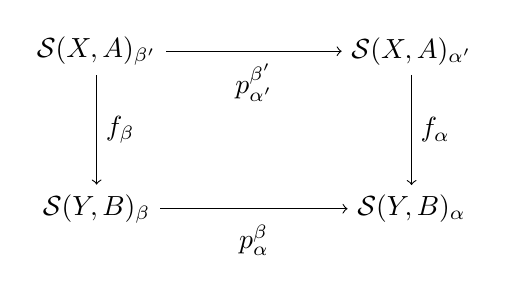
\begin{tikzpicture}
	
	
	
	\node (w) at (0,0) {\(\mathcal{S}(X,A)_{\beta'}\)};
	
	\node (x) at (0,-2) {\(\mathcal{S}(Y,B)_{\beta}\)};
	
	\node (y) at (4,-2) {\(\mathcal{S}(Y,B)_{\alpha}\)};
	
	\node (z) at (4,0) {\(\mathcal{S}(X,A)_{\alpha'}\)};
	
	\node (f) at (2,-2.4){\(p^\beta_\alpha\)};
	
	\node (g) at (2,-0.4){\(p^{\beta'}_{\alpha'}\)};
	
	\node (s) at (0.3,-1) {\(f_{\beta}\)};
	
	\node (s2) at (4.3,-1) {\(f_{\alpha}\)};	
	
	\draw[->] (z) -- (y);
	\draw[->] (w) -- (x);
	\draw[->] (x) -- (y);
	\draw[->] (w) -- (z);
	
	
	\end{tikzpicture}
	$$

\end{lem}

\begin{proof}
Let $\{U_i\}_{i \in J}$ be some simplex in $\mathcal{S}(X,A)_{\beta'}$. For every edge $U$ the set $f^{-1} \circ p \circ f(U) $ is non-empty because $p$ maps $f(U)$ to larger set. Thus for every edge $U_i$ there is corresponding edge in $\mathcal{S}(X,A)_{\alpha'}$. We can now define map $p^{\beta'}_{\alpha'}: \mathcal{S}(X,A)_{\beta'} \rightarrow \mathcal{S}(X,A)_{\alpha}$ in such way that edge $U$ is mapped to the edge $f^{-1}pfU $ and we extend this map by linearity. Now by defining map $p^{\beta'}_{\alpha'}$ in such way for every simplex we get well-defined map for which the diagram commutes.
\end{proof}

\chapter{Cech homology}

In this chapter we will construct Cech homology and prove main results related to it.  We will first define inverse system of homology groups of the nerves.

\begin{maar}
Let $\alpha$ be element of COV$(X,A)$ and $G$ abelian group. Then we can define group $H_{q,a}(X,A;G)$ using the singular homology groups in a following way: $$H_{q,a}(X,A;G) = H_q(\mathcal{S}(X,A)_{\alpha};G)$$. 
For every coverings of $\alpha, \beta$ in $(X,A)$ for which $\alpha \leq \beta$ we define the maps to be
$$I^{\beta}_{\alpha}: H_{q,\beta} \rightarrow  H_{q,\alpha}$$ 
maps $I_{\beta}^{\alpha}$ are induced by some maps $p^\beta_\alpha$ which are unique up to homotopy.
\end{maar}
\begin{lem}
Let $q \in \N$ be fixed number, let $(X,A)$ be topological pair and $G$ abelian group. Then groups $H_{q,a}(X,A;G)$ together with maps $I_{\beta}^{\alpha}$ form inverse system of groups.
\end{lem}
\begin{proof}
First we have to show that $I_{\alpha}^{\alpha}$ is identity function for every $\alpha \in$ COV$(X,A)$. We already know that identity map between simplicial complexes is projection map and because identity map induces identity map between the complexes by uniqueness of $I_{\alpha}^{\alpha}$ we see that the map has to be identity map between corresponding homology groups.\newline Now for every coverings $\alpha, \beta, \gamma$ of pair $(X,A)$ for which relation $\alpha \leq \beta \leq \gamma$ holds we have to show that $I_{\beta}^{\gamma} \circ I_{\alpha}^{\beta} = I^{\gamma}_{\alpha}$. By lemma \ref{compofprojmaps} the composition of corresponding projection maps $p_{\beta}^{\gamma} \circ p_{\alpha}^{\beta}$ is projection map. Thus it defines map $I^{\gamma}_{\alpha}$.
\end{proof}
Now we are ready to define the cech homology groups $ \check{\mathrm{H}}_n$.
\begin{maar}
Let $(X,A)$ be topological pair and $G$ abelian group. Then cech homology groups with coefficients $G$ are defined to be inverse limits of $H_{q,\alpha}(X,A;G)$ where $\alpha$ belongs to COV$(X,A)$. Simply denoted  $\check{\mathrm{H}}_q(X,A;G) = \lim_{\rightarrow}\{H_{q,\alpha}(X,A;G)\}$

\end{maar}
Because coverings can be infinite the limits are not necessary defined. However there is a way to evade this problem. 

\section{Well-definedness of the Cech homology groups}
In this section we will provide condition for the spaces which will guarantee that the Cech groups are well-defined. 
...
From now on in this chapter we assume that the topological spaces are such for which the Cech groups  are well-defined. 

\section{Induced homomorphisms}
In this section we will investigate properties of induced homomorphism. Earlier we defined Cech homology groups to be limit of the groups induced by coverings of the pair. In section \ref{limitmorphism} we defined concept of limit homomorphism. In next theorem we will show that such homomorphism exists.

\begin{lause}
Let $f:(X,A) \rightarrow (Y,B)$ be continuous function between pairs of spaces. Let $\mathcal{A} = \{f_\alpha \mid \alpha \text{ is covering of pair }(Y,B)\}$ be family of functions for which every element of the open covering $\alpha$ is mapped to its preimage. This family induces maps between corresponding cech homology groups. $$f'_{\alpha,q}:H_q(\mathcal{S}(X,A)_{f^{-1}\alpha}) \rightarrow H_q(\mathcal{S}(Y,B)_{\alpha})$$
We denote family of functions described above with $\mathcal{A}_q$ . Then every such collections is natural transformation of the Cech homology groups and thus the limit function is well defined. 
\end{lause}
\begin{proof}
We can define function $\phi:\text{COV}(Y,B) \rightarrow \text{COV}(A,B)$ to map every set $U$ of $\alpha$ to set $f^{-1}U$ of $f^{-1}\alpha$. By lemma \ref{preimageorder} this map preserves order. Let $\beta$ and $\alpha$ be some coverings of pair $(Y,B)$. We denote $\alpha'$ and $\beta'$ to be preimages of $\alpha$ and $\beta$ under map $f$. The diagram of lemma \ref{squarelemmaforcoverings} shows that the corresponding maps between coverings commute. Thus we have following commutable diagram:
	$$
	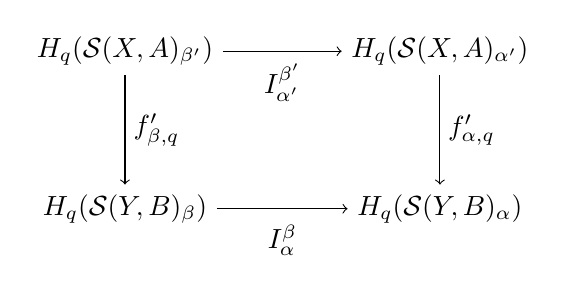
\begin{tikzpicture}
	
	
	
	\node (w) at (0,0) {\(H_q(\mathcal{S}(X,A)_{\beta'})\)};
	
	\node (x) at (0,-2) {\(H_q(\mathcal{S}(Y,B)_{\beta})\)};
	
	\node (y) at (4,-2) {\(H_q(\mathcal{S}(Y,B)_{\alpha})\)};
	
	\node (z) at (4,0) {\(H_q(\mathcal{S}(X,A)_{\alpha'})\)};
	
	\node (f) at (2,-2.4){\(I^\beta_\alpha\)};
	
	\node (g) at (2,-0.4){\(I^{\beta'}_{\alpha'}\)};
	
	\node (s) at (0.4,-1) {\(f'_{\beta,q}\)};
	
	\node (s2) at (4.4,-1) {\(f'_{\alpha,q}\)};	
	
	\draw[->] (z) -- (y);
	\draw[->] (w) -- (x);
	\draw[->] (x) -- (y);
	\draw[->] (w) -- (z);
	
	
	\end{tikzpicture}
	$$
	
The fact that collection $\mathcal{A}_q$ is natural transformation of the groups follows directly from the above diagram. Thus by lemma \ref{limitmorphismgroup} there exists limit homomorphism $$f_q:\check{\mathrm{H}}(X,A;G) \rightarrow \check{\mathrm{H}}(Y,B;G) $$
\end{proof}



\section{Dimension axiom}
In this section we will prove that the cech homology theory satisfies the dimension axiom.




\begin{thebibliography}{9}

\bibitem{Rotman}\label{rotman}

J. Rotman An Introduction to Algebraic Topology (Graduate Texts in Mathematics), Springer 

\bibitem{First}
L. G�rniewicz, Topological Fixed Point Theory of Multivalued Mappings, Kluwer Academic
Publishers, 1999.

\bibitem{Second} 
I. L. Glicksberg, A further generalization of the Kakutani fixed point theorem with
application to Nash equilibrium points, Proc. Amer. Math. Soc. 3 (1952), 170�174.


\bibitem{Vaisala}\label{vai}
M. BAYE, G. TIAN, ANU J. ZHOU, �The Existence of Pure Nash Equilibrium in Games 
with Nonquasiconcave Payoffs,� Texas A  M University, mimeo, 1990. 

\bibitem{categorytheory}
Saunders Mac Lane: Categories for the Working Mathematician (Graduate Texts in Mathematics)

\bibitem{algebra2}\label{algebra2}
Jokke H�s�: Algebra II, 2016. 

\end{thebibliography}

\end{document}
